\documentclass[11pt,twoside,a4paper]{article}

\usepackage{url}
\usepackage{fixltx2e}
\usepackage{amsmath}
\usepackage{amsfonts}
\usepackage{graphicx}
\usepackage{amssymb}
\usepackage{multicol}
\usepackage{listings}
\usepackage{mdwlist}

% \textsubscript{}
% \textsuperscript{}

\begin{document}
  
  \graphicspath{{img//}}
  
  \title{Maths for Informatics: 4b Geomatry \\Revision Notes \\ Ver 0.1}
  \author{Guy Taylor}
  \date{April 2011}
  
  \maketitle
  
  \tableofcontents
  
  \section{Introduction}
    This document is a set of revision notes for the Geomatry for Informatics course at the Univerisy of Edinbugh.
  
  \clearpage
  \section{Mapping}
    \subsection{Matrix}
      If a matrix is arthoginal in \(\mathbb{R}^3\) on can show that \(MM^T = I\) then:
      \begin{description}
        \item[If \(det(m) = 1\)] \hfill \\
          This ia a rotation around some line \(L \in \mathbb{R}^3\) that passes through \(0 (0,0,0)\) at angle \(\alpha\).
          
          If you find the \textit{Eigan Vector} that is a line parralles to \(L\), set it to \((0,0,0)\) and we have the line.
        
        \item[If \(det(m) = -1\)] \hfill \\
          This is a reflection in a plane.
      \end{description}
  
  \section{Shapes}
    \begin{tabular}{l|l|l}
      \textbf{Example}  & \textbf{Name} & \textbf{Visual Representation} \\ \hline
      \(x^2+y^2+z^2=1\) & Sphere        & 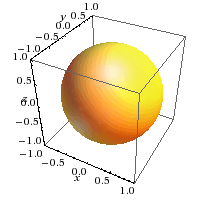
\includegraphics[width=2cm]{MSP195419f85bd4320b17g400004245ieica2347c33}\cite{sphere_graphic} \\
      \(x^2+y^2=z^2\)   & Conic         & 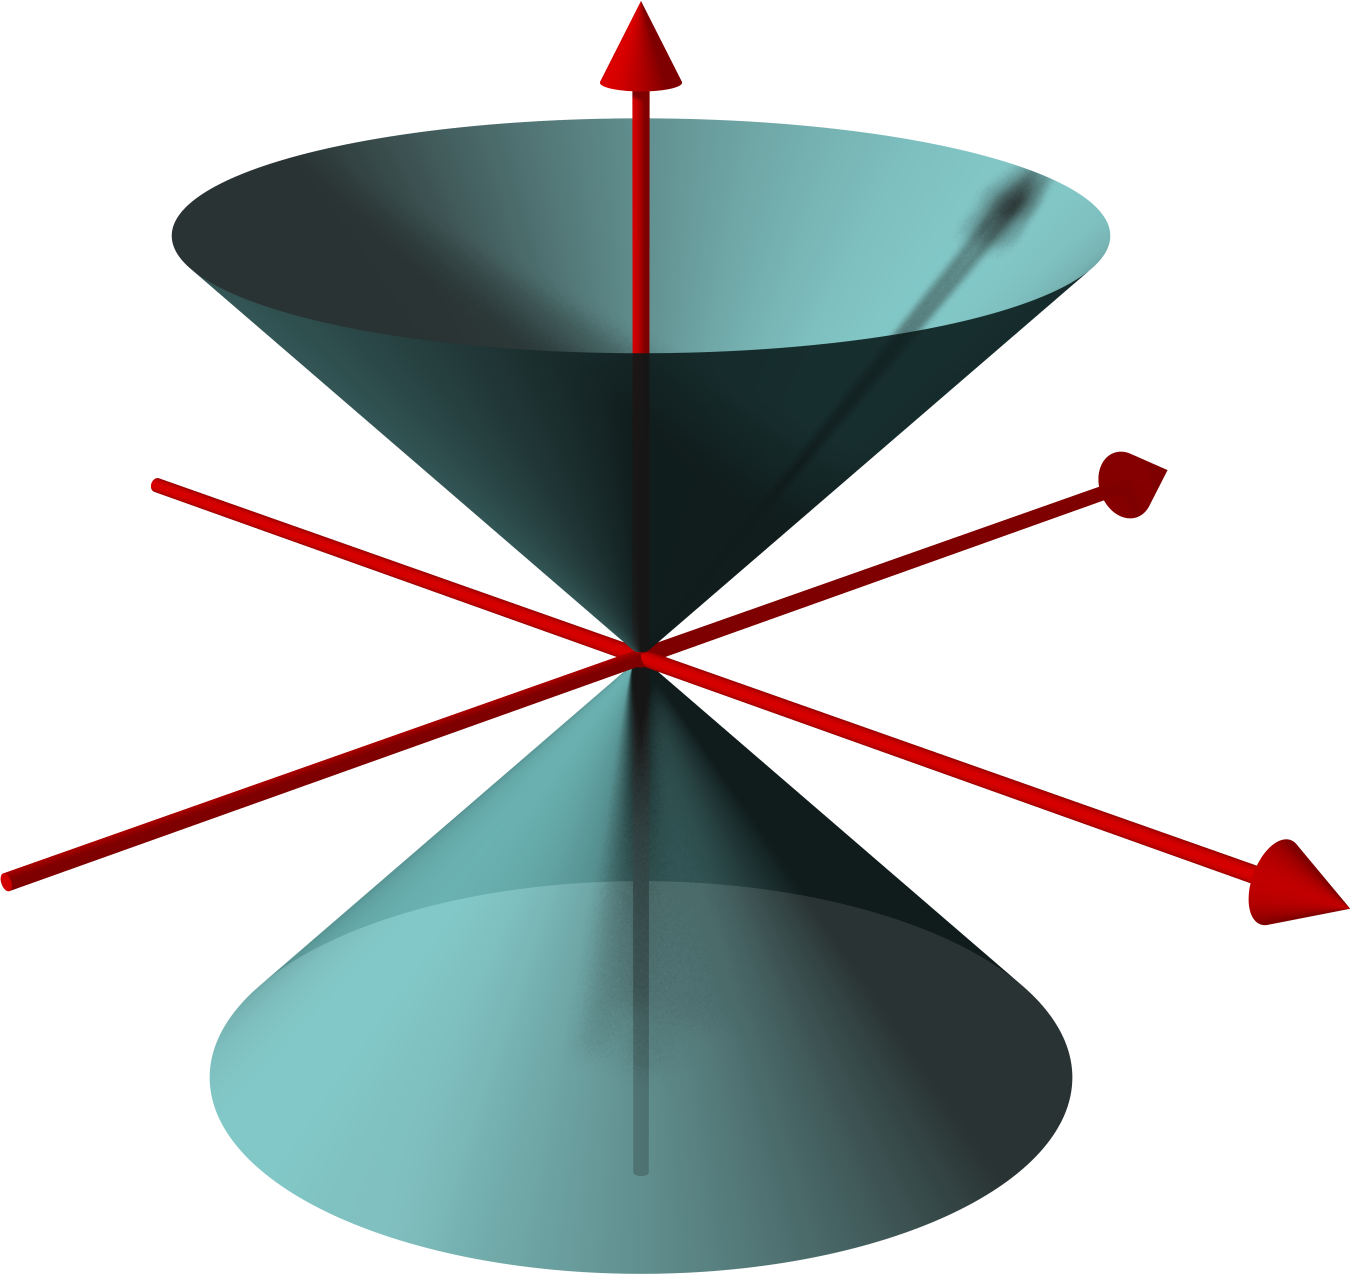
\includegraphics[width=2cm]{DoubleCone} \\
      \(x^2+y^2=z\)     & Poraboloid    & 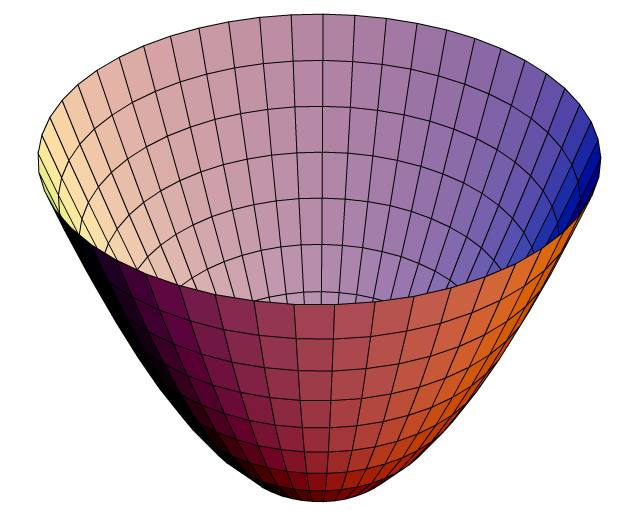
\includegraphics[width=2cm]{Paraboloid_of_Revolution}  \\
    \end{tabular}
    
    \subsection{Types}
      \begin{description}
        \item[Ellipse] \hfill \\
          \[ \frac{x^2}{a^2} + \frac{y^2}{b^2} = 1 \]
        
        \item[Hyperbola] \hfill \\
          \[ \frac{x^2}{a^2} - \frac{y^2}{b^2} = 1 \]
        
        \item[Parabola] \hfill \\
          \[ y^2 = 4ax \]
        
        \item[Other] \hfill \\
          \begin{tabular}{l|l|l}
            Union of two line &                          & \(  \)       \\ % TODO
            Line              & Shortest distance between two points & \( y=Mx+c \) \\
            Point             & A zero dimensinal object & \( (x,y) \)  \\
            Empty             & Nothing                  & \( \{\} \)   \\
          \end{tabular}
      \end{description}
    
    \subsection{Generalisation}
      \[ Ax^2 + Bxy^2 + Cy^2 + Dx^2 + F = 0 \]
      or
      \[
        \begin{bmatrix} x & y \end{bmatrix}
        \begin{bmatrix}
          A           & \frac{B}{2} \\[0.3em]
          \frac{B}{2} & C
        \end{bmatrix}
        \begin{bmatrix} x \\ y \end{bmatrix}
        +
        \begin{bmatrix} x & y \end{bmatrix}
        \begin{bmatrix} D \\ E \end{bmatrix}
        + F = 0
      \]
    
    \subsection{Idetification}
      \[
        N =
          \begin{bmatrix}
            A           & \frac{B}{2} & \frac{D}{2} \\[0.3em]
            \frac{B}{2} & C           & \frac{E}{2} \\[0.3em]
            \frac{D}{2} & \frac{E}{2} & F           \\
          \end{bmatrix}
        M =
          \begin{bmatrix}
            A           & \frac{B}{2} \\[0.3em]
            \frac{B}{2} & C
          \end{bmatrix}
      \]
      \begin{description}
        \item[Ellipse] \hfill \\
          \( 4AC - B^2 > 0 \) and \( det(N)(A+C) < 0 \)
        
        \item[Hyperbola] \hfill \\
          \( 4AC - B^2 < 0 \) and \( det(N) \neq 0 \)
        
        \item[Parabola] \hfill \\
          \( 4AC - B^2 = 0 \) and \( det(N) \neq 0 \)
      \end{description}
  
  \clearpage
  \section{Examples}
  
    \subsection{Example 1}
      \label{Example_1_1}
      Note: Simmilar to assignment
      \begin{description}
        \item[Question] \hfill \\
          \(
            S:x^2+y^2-z^2=1 \\
            S\subset\mathbb{R}^3 \\
          \)
          If you are given a point and asked to find all lines that pass through it\\
          Hint: There will allways be two
        
        \item[Answer] \hfill \\
        %\begin{multicols}{2}
          \(
            pt(1,1,1) \\*
            P \leq L \leq S \subseteq \mathbb{R}^3 \\
            L = (1+a\alpha, 1+b\alpha, 1+c\alpha) \\
          \)
            \\ Inserted into questions formula \\
          \(
            (1+a\alpha)^2 + (1+b\alpha)^2 + (1+c\alpha)^2 = 1  \forall \alpha \\
          \)
            \\ Expand to\\
          \(
            1+ ... = 1 \\
          \)
            \\ seperate varibles \\
          \(
            \alpha(2a+2b-2c)+\alpha^2(a^2+b^2-c^2) = 0 \\
          \)
            \\ Divide by \(\alpha\) \\
          \(
            (2a+2b-2c) = 0 or (a^2+b^2-c^2) = 0 \\
          \)
            \\ let a = 1 (as 1 is modulo all numbers) \\
          \(
            (1,b,c) \\
            1+b^2-c^2 = 0 and 1+b-c=0 \\
            b=0 and c=1 \\
          \)
            \\ Form to a equation \\ (are intial point and are new derived point) \\
          \(
            \underline{(1,1,1) + \alpha(1,0,1)}
          \)
        %\end{multicols}
      \end{description}
  
  \clearpage
  \section{Matrix and Vector}
    \subsection{Matrix}
      TODO
    
    \subsection{Vector}
      TODO
    
    \subsection{Mix}
      \begin{tabular}{ll}
        \textbf{Orthoginal}    & $ a \cdot b = 1 $ \\ \\
        \textbf{Parrallel}     & $ a \cdot b = 0 $ \\ \\
        \textbf{Cross Product} & $
          \begin{vmatrix}
            i   & j   & k   \\
        	  a_1 & a_2 & a_3 \\
        	  b_1 & b_2 & b_3 \\
        	\end{vmatrix} $ \\ \\
        \textbf{Dot Product}   & $ (a_1xb_1) + (a_2xb_2) + (a_2xb_2) $ \\ \\
        \textbf{Angle}         & $ cos(\theta) = \frac{a \cdot b}{|a||b|} $ \\ \\
        \textbf{Determinate}   & $ \begin{vmatrix} a & b \\ c & d \end{vmatrix} = ad - bc $ \\ \\
        \textbf{Determinate}   & $
        	  \begin{vmatrix}
        	    a & b & c \\
        	    d & e & f \\
        	    g & h & i \\
        	  \end{vmatrix}
        	  =
        	  \begin{matrix}
        	    a & b & c & \nearrow \\
        	    d & e & f & \nearrow & Y \\
        	    g & h & i & \nearrow \\
        	    a & b & c & \searrow \\
        	    d & e & f & \searrow & X \\
        	    g & h & i & \searrow \\
        	  \end{matrix}
        	  X-Y $ \\ \\        	
        \end{tabular}
  
  \clearpage  
  \begin{thebibliography}{9}
    \bibitem{sphere_graphic}
        "Sphere Graphic", Author="Wolfram|Alpha", Publisher"Wolfram Alpha LLC", Accessed="26-April-2011", Year="2011", "\url{http://www.wolframalpha.com/input/?i=x^2%2By^2%2Bz^2%3D1}"
  \end{thebibliography}
    
\end{document}
